\section{Test Site}
%%%%%%%%%%%%%%%%%%%%%%%% FRAME 0 %%%%%%%%%%%%%%%%%%%%%%%%%%%%%%%
{
	\setbeamertemplate{footline}{}
	\begin{frame}
		\begin{tikzpicture}[remember picture,overlay]
			\node[at=(current page.center)] {
				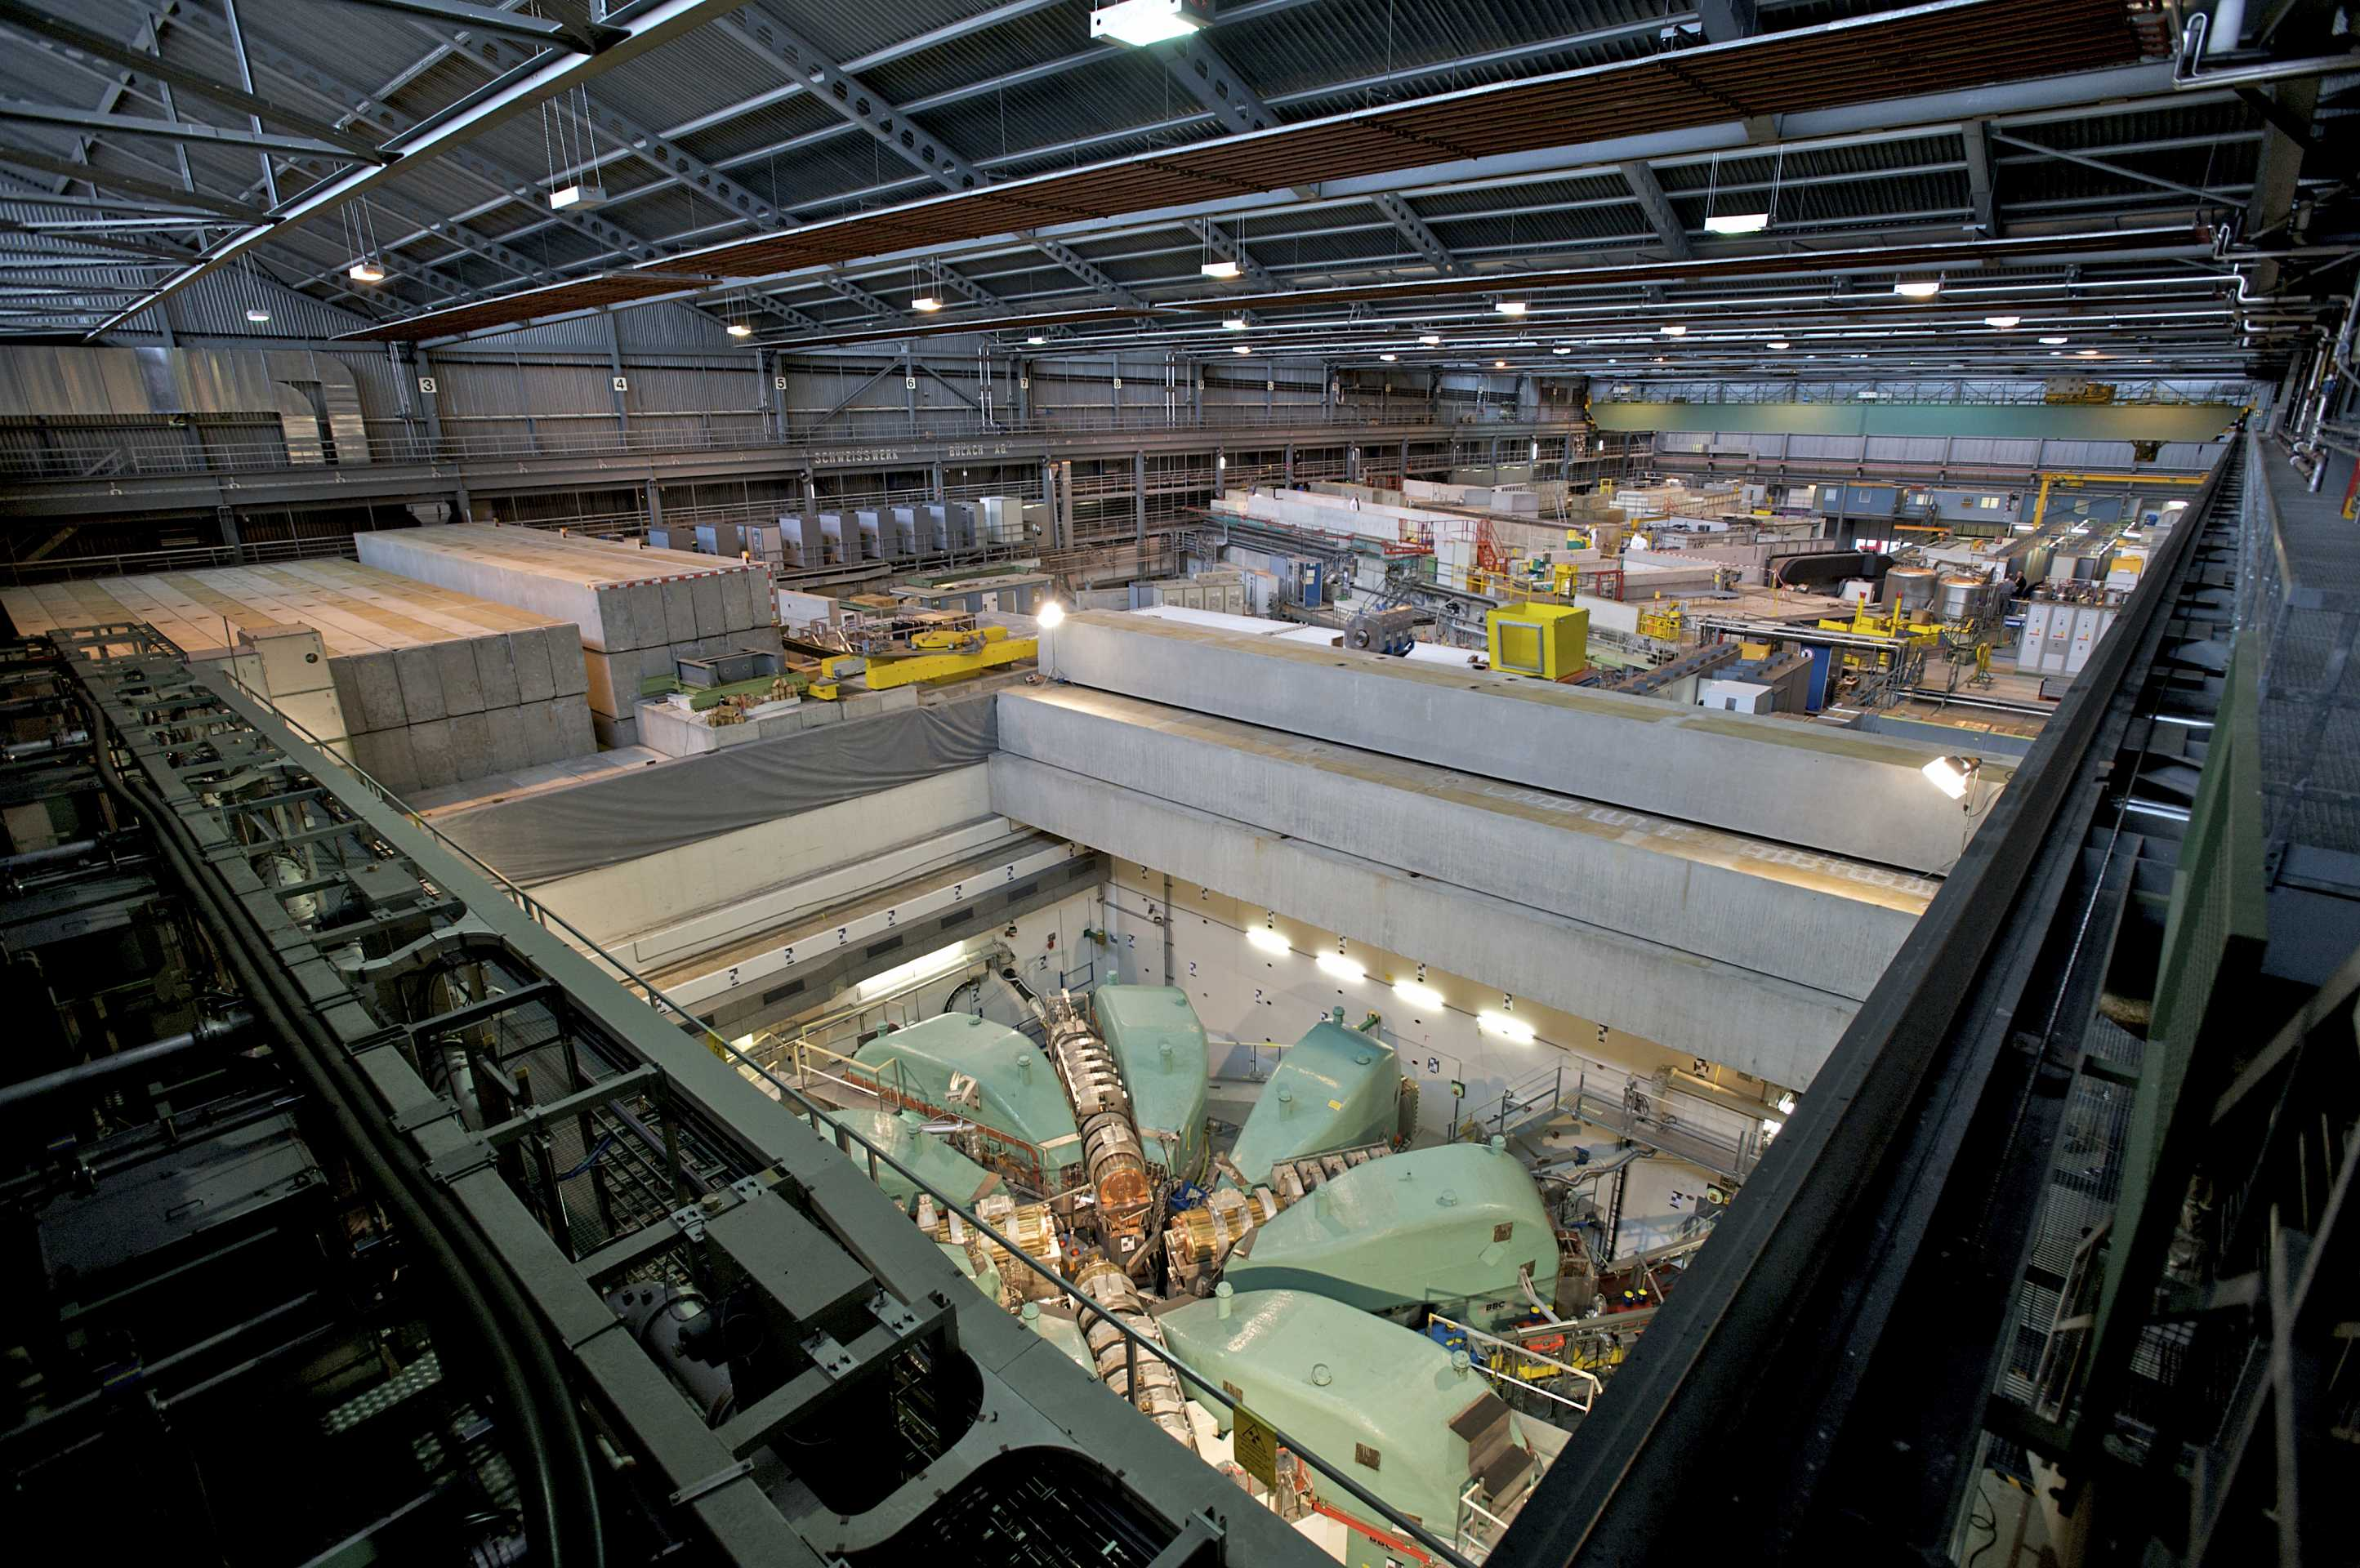
\includegraphics[width=1.15\paperwidth]{Cyclo2}};
		\end{tikzpicture}
		
	\end{frame}
}
%%%%%%%%%%%%%%%%%%%%%%%% FRAME 1 %%%%%%%%%%%%%%%%%%%%%%%%%%%%%%%
\subsection{PSI Experimental Hall}
\begin{frame}{Test Site}

    \vspace*{-10pt}
	\begin{itemize}\itemfill
		\item High Intensity Proton Accelerator (HIPA) at PSI (Cyclotron) \ra beam line PiM1 
		\item clean positive pion beam (\SI{\sim98}{\%} $\uppi^+$) with momentum of \SI{260}{\mega\electronvolt\per c} 
		\begin{itemize}
			\item \sfrac{3}{4} smaller signals than at CERN! (\SI{120}{\giga\electronvolt\per c})
		\end{itemize}
		\item \good{tunable particle fluxes from \orderof{\SI{1}{\kilo\hertz\per cm^2}} to \orderof{\SI{10}{\mega\hertz\per cm^2}}}
		\item \bad{significant multiple scattering \ra worsens resolution}
	\end{itemize}
	
	\subfigs[\subfig[.36]{.48}{Cyclo1}]{\subfig[.3]{.5}{Cyclo3}}{\subfig[.22]{.25}{Target}}\vspace*{-10pt}

\end{frame}
